\documentclass[10pt]{article}

% amsmath package, useful for mathematical formulas
\usepackage{amsmath}
% amssymb package, useful for mathematical symbols
\usepackage{amssymb}

% graphicx package, useful for including eps and pdf graphics
% include graphics with the command \includegraphics
\usepackage{graphicx}

% cite package, to clean up citations in the main text. Do not remove.
\usepackage{cite}

\usepackage{color} 

% Use doublespacing - comment out for single spacing
\usepackage{setspace} 
\doublespacing

% Text layout
\topmargin 0.0cm
\oddsidemargin 0.5cm
\evensidemargin 0.5cm
\textwidth 16cm 
\textheight 21cm

% Bold the 'Figure #' in the caption and separate it with a period
% Captions will be left justified
\usepackage[labelfont=bf,labelsep=period,justification=raggedright]{caption}

% Use the PLoS provided bibtex style
\bibliographystyle{plos2009}

% Remove brackets from numbering in List of References
\makeatletter
\renewcommand{\@biblabel}[1]{\quad#1.}
\makeatother


% Leave date blank
\date{}

\pagestyle{myheadings}
%% ** EDIT HERE **


%% ** EDIT HERE **
%% PLEASE INCLUDE ALL MACROS BELOW

\usepackage{multirow}
\renewcommand{\arraystretch}{1.1}

% figure files reside in the figures/ directory
\graphicspath{
{figures/}
}

%% END MACROS SECTION

\begin{document}

% Title must be 150 characters or less
\begin{flushleft}
{\Large
\textbf{Spatially explicit model of the lymphocyte diaspora in influenza-infected lung quantifies constraints of chemokine directed migration}
}
% Insert Author names, affiliations and corresponding author email.
\\
Drew Levin$^{1,\ast}$, 
Stephanie Forrest$^{1}$, 
Soumya Banerjee$^{1}$
Candice Clay$^{2}$, 
Melanie Moses$^{1}$, 
Frederick Koster$^{1,2}$, 
\\
\bf{1} Department of Computer Science, University of New Mexico, Albuquerque, NM, USA
\\
\bf{2} Lovelace Respiratory Research Institute, Albuquerque, NM, USA
\\
$\ast$ E-mail: Corresponding drew@cs.unm.edu
\end{flushleft}



% Please keep the abstract between 250 and 300 words
\section*{Abstract}

During the primary immune response, clearance of influenza in the lung requires the homing of activated CD8 T cells during the lymphocyte diaspora from regional lymph nodes to small infected foci comprising a tiny fraction of the total lung.  T cell navigation to the infected region is undirected but focused migration is made possible by local cytokine and chemokine production from infected epithelial cells.  We examined the efficiency of local chemokines to induce migration of activated CD8 T cells using simulations in a purpose-built agent-based mathematical model (CyCells).  

Avian H5N1, seasonal H1N1, and 2009 pandemic influenza strains were used separately to induce chemokine production \textit{in vitro}.  Of the chemokines tested, only secretion of CXCL10 (IP-10) and CCL5 (RANTES) was stimulated by infection with these three influenza strains, with IP-10 dominating the directed migration due to higher concentrations.  A delayed differential equation model was fit to the empirical per cell chemokine production rates, coupled with published T cell migration parameters, to calibrate the spatially explicit model in order to test inter-strain variation on T cell recruitment in the lungs.  We observe that T cell sensitivity to chemokine is just high enough to maximize their efficiency.  The modeled immune response is unable to clear the pandemic strain due to its high rate of viral production and large plaque size.  

The spatial nature of the model reveals unique challenges to T cell recruitment and motility not visible in spatially homogeneous ODE models.  Expanding plaque sizes isolate infected cells, impeding T cell discovery and infection control. In the model, T cells executed an efficient search with high sensitivity to either chemokine detected. A key limitation imposed on T cells was illustrated in their failure to clear the most rapidly replicating pandemic H1N1 virus after day 6, when T cells became ‘lost’ and inefficient in large infected foci as revealed in cinematic displays. This spatially explicit model is consistent with an efficient T cell recruitment to infected lung, without apparent means to induce increased efficiency, leaving vaccination as the key to shortening the interval between initial infection and T cell activation.

% Please keep the Author Summary between 150 and 200 words
% Use first person. PLoS ONE authors please skip this step. 
% Author Summary not valid for PLoS ONE submissions.   
\section*{Author Summary}

Seasonal influenza infects up to 10,000,000 people and kills between 250,000 and 500,00 people every year.  Recent mutant strains of flu with high morbidity such as Avian H5N1 and 2009 Pandemic H1N1 raise the possibility of a global pandemic in the near future.  In order to clear an infection in the lung, T cells produced in the lymph nodes must navigate the branching bronchial vascular system in order to reach the site of infection.  Using an agent-based model, we look at how molecular signaling by cells infected with three differing strains of influenza aid this search process.  Our experimental data shows that two chemokines, IP-10 and RANTES, are help improve T cell search.  The spatial nature of our model reveals challenges to this search process not seen in conventional ordinary differential equation (ODE) models.  The simulated immune response is not able to contain the highly virulent 2009 pandemic H1N1 strain, suggesting that early intervention, i.e. vaccination, is key to containing the infection.

\section*{Introduction}

The adaptive immune response induced during acute influenza A infection is a complex web of defense mechanisms that controls all but the most virulent strains.  Understanding its components and their interactions are relevant to improving vaccines and strategies to control immunopathology. Elegant studies in the mouse model have described the induction and effector phases of the adaptive immune response, including functional capabilities of the innate interferon-directed response, macrophages, specific antibody, and cytotoxic effector lymphocytes \cite{Sallusto2000, Joo2008, Mackay2008}.   CD8+ T cells are necessary for the resolution of pneumonia and complete clearance of mouse-adapted influenza strains \cite{Sallusto2000, Joo2008, Mackay2008, Miao2010}, but gaps remain in our understanding of the behavior of activated T cells in infected tissue.

The generally held view of the sequence of CD8+ T cell events during a primary immune response to influenza in the lung involves the following steps: dendritic cells bearing specific antigen migrate from the lung to the draining lymph node where naive T and B cell precursors are activated in specialized architecture \cite{Saenz2010, Beltman2007, Handel2008, Zheng2008, Ingulli2009, Allan1990}.  T cells proliferate in the lymph node and are released into the bloodstream, appearing simultaneously in the lung, spleen and other organs 4-5 days post-infection, a whole-body distribution known as the lymphocyte diaspora \cite{Thelen2008}.  In the lung, extravasation from capillaries is signaled by inflammatory cytokine-mediated integrin-activation on endothelial cells.  Once in the tissue, T cells follow a chemokine gradient to the infected epithelial cells secreting the chemokine.

Mathematical models have used detailed mouse data to characterize the evolution of the immune response and predict its impact on viral kinetics \cite{Thomas-Vaslin2008, Beauchemin2008, Smith2010, Thakar2010, Burrowes2004}.  Such whole-response modeling has considerable potential to inform strategies of vaccination and therapy, thus avoiding subsequent expensive animal and human trials.  Models using ordinary differential equations to predict temporal events, however, do not account for spatial constraints, and must make assumptions about the efficiency of the viral spread and interaction of different populations. 

Here we study the time and physical constraints of the lymphocyte diaspora using an agent-based model (ABM).  To develop a model with tractable simulations, some components of host defense are abstracted and the model therefore does not aim to predict the true outcome for each strain examined.   We ask how very small foci of infected tissue can attract limited numbers of activated CD8 T cells after release into the systemic vascular system.  The circulating blood supply services non-infected tissue orders of magnitude larger than the target infected tissue, necessitating an efficient mechanism to focus cell migration.   A host of cytokines and chemokines secreted by infected cells are critical in directing immune cells to sites of infection \cite{Miao2010, Zhao2000, LiJeon2002}.  While each chemokine has been studied in detail for receptor specificity and function in knockout models, the local advantage brought by chemokine secretion in an inflammatory context have not been examined in detail in a virus-infected whole animal model.  

To characterize the local chemokine-secretion environment in which T cells migrate, we used data on viral secretion and chemokine secretion patterns from human epithelial cells infected in vitro by three different influenza virus strains of avian, seasonal and pandemic origins \cite{Mitchell2011}.   We selected in vitro chemokine data as a tissue environment surrogate, because it may be more accurate than published chemokine levels in mouse blood and bronchial alveolar fluid, and it allowed us to represent sustained chemokine gradients within the model lung.  Extensive literature on mouse model data of infections with mouse-adapted strains PR8 and HK-31 were used to calibrate the ABM model. [REF]

The standard hypothesis posits that the marked strain-specific differences in replication efficiency and tissue spread previously reported \cite{Mitchell2011} would largely determine the outcome of infection as eradication or lack of control.  Our model confirms this hypothesis, but we also observed three interesting characteristics of chemokine-directed migration not revealed by earlier data.  First, of the only two chemokines stimulated by all three strains, the influence of IP-10 consistently dominated the effect of RANTES, regardless of strain.  Second, each chemokine exhibited a clear threshold to direct migration, with diminishing improvements at increasing concentrations above the threshold.  Finally, when the target (infection focus) was large, T cell search became inefficient due to the disappearance of the chemokine gradient, possibly contributing to the loss of control of the pandemic strain.  

% You may title this section "Methods" or "Models". 
% "Models" is not a valid title for PLoS ONE authors. However, PLoS ONE
% authors may use "Analysis" 
\section*{Models}


\subsection*{Computational Modeling}


Computational modeling used CyCells \cite{Warrender2006}, a modeling platform for two- or three-dimensional agent-based simulations of the immune response. A simplified model of T cell activation and recirculation was implemented in CyCells (Fig.~\ref{fig:modelchart}), and simulations measured efficiency of infection clearance under different environmental conditions. The lung was represented as a two-dimensional sheet of healthy epithelial cells. Vasculature was represented as a binary tree with fourteen branches originating at a single lymph node. Activated T cells descend through the vascular tree until cytokine signal is detected on the local endothelium, at which point they exit the vasculature and follow the chemotactic gradient to the site of infection. T cells that do not encounter cytokine recirculate to the lymph node. At the site of infection when a T cell encounters an infected epithelial cell it induces apoptosis.

The simulation begins when a single cell in the center of the tissue is infected. After the eclipse phase (incubation), the infected cell begins secreting virus and chemokine. Virus diffuses locally, infecting nearby cells, and continuing the cycle. Chemokine diffuses from secreting cells, creating a ball of stimulation around the infected region. After a five day delay to simulate lymph node stimulation and T cell proliferation, activated T cells exit the lymph node and circulate through the vasculature to the tissue. Because T  cells cannot choose their path through the branching network, we assume they arrive in tissue at random locations. 


\subsection*{Model Definition}

In the model, epithelial cells are stationary and can be in one of five different states: \emph{healthy}, \emph{virus-incubating}, \emph{virus-expressing}, \emph{apoptotic}, and \emph{dead}. \emph{Healthy} cells remain unchanged unless infected by virus. Once infected, the cell transitions from {incubating} to \emph{expressing}. \emph{Expressing} cells secrete virus and chemokine for approximately 17 hours and then die. \emph{Expressing} cells become \emph{apoptotic} if they encounter activated T cells. Apoptoic cells continue to secrete virus until they die one hour after their transition. \emph{Dead} cells remain inert and do not regenerate over the course of an infection.

T cells have three states. \emph{Circulating} T cells begin to emerge from the lymph node at five days post infection. \textit{Emigrating} T cells arrive at a random location on the lung's surface, wander randomly in the tissue for 10 minutes, and transition to \emph{circulating} in the absence of chemokine. \emph{Circulating} cells spend six minutes recirculating to the lymph node, transition to \emph{emigrating} and are reintroduced to a new random location in the lung. When a \emph{emigrating} T cell encounters chemokine, it converts to \emph{chemotaxing} and begins following the chemotactic gradient to the source of infection. \emph{Chemotaxing} T cells move continuously up the gradient, inducing apoptosis if they encounter \emph{expressing} epithelial cells. \emph{Chemotaxing} cells decay exponentially with an average lifespan of two hours. 

The model contains two kinds of particles: virus and chemokine. Both are produced at constant rates by \emph{expressing} epithelial cells.  Virus diffuses through the lung tissue, infecting healthy cells probabilistically according to the local virus concentration. Chemokine diffuses across the tissue but has no
direct effect beyond activating T cells. Both particle types decay exponentially.

Parameters that are consistent between every model are shown in Table \ref{table:parameters}.  Strain-specific values are shown in Table \ref{table:strains}.

\section*{Materials}

Chemokine secretion:  Epithelial cell culture and supernatant collection was performed as described \cite{Mitchell2011}.  Briefly, undifferentiated human tracheal epithelial cells (University of Miami) were cultured for 4 weeks to achieve fully differentiated confluent monolayers on collagen-coated transwell inserts, or commercial differentiated human bronchial epithelial cells (EpiAirway Tissue, MatTek Corp., Ashland, MA) used immediately upon receipt, were infected at an MOI of 0.01 with either seasonal H1N1 virus A/New Caledonia/20/99 (sH1N1), the 2009 H1N1 pandemic strain A/California/04/09 (pH1N1), or avian H5N1 virus A/Hong Kong/483/97 (aH5N1) derived from a fatal human infection.  Apical fluid for viral secretion, and basal media for chemokine secretion collected before treatment of the monolayer with protease, was collected from previously undisturbed triplicate or quadruplicate wells at 0, 6, 10, 12, 16, 20, 24, 30, 36, 42, 48, and 72 hours after infection, and stored at -80C until assay.  Quantitative viral culture was performed by standard plaque assay.  Quantitative chemokine levels were performed in 30 µl aliquots for a panel of chemokines (IL-8, MCP-1, MIP-1$\alpha$, MIP-1$\beta$, RANTES, IP-10, eotaxin) and cytokines (interferon-gamma, IL-1$\alpha$, IL-1$\beta$, IL-1RA, IL-2, IL-3, IL-4, IL-6, IL-10, IL-12p40, IL-15, IL-17, TNF$\alpha$) (Luminex Assay®, Luminex Corp.) and reported as ng/mL basal media sampled from a total volume of 4 mL.  Only IP-10, RANTES, and TNF$\alpha$ showed increases in production.  TNF was ignored as its effects are outside the scope of this paper.


% Results and Discussion can be combined.
\section*{Results}

\subsection*{Chemokine production}

Chemokine data were collected from epithelial monolayers infected with three different influenza strains, as described in \cite{Mitchell2011} (Fig.~\ref{fig:data}).  IP-10 concentration increases were observed by 8h post-infection (p.i.), and RANTES by 16h p.i..  To estimate per-cell production rates, we extended the ODE model of Ref. \cite{Mitchell2011} to represent chemokine production from infected cells (Eq. \textbf{S}1).  Model fits, (Table \ref{table:strains}), were computed for three strains (Fig.~\ref{fig:data}) using Matlab's \texttt{nlinfit} function (Levenberg-Marquardt algorithm).  The resulting chemokine production values were used in the CyCells ABM.  Best-fit expression rates were similar for all strains except for significantly higher RANTES production in aH5N1.  There is no positive correlation between viral production and induced chemokine production across the three strains.


\subsection*{T cell sensitivity to chemokine}

The model uses chemokine gradient as a surrogate for the inflammatory cytokines required for extravasation.  Figure \ref{fig:cycells} shows chemokine concentrated around virus secreting cells.  However, T cell sensitivity determines how strong the aggregate chemokine signal must be.

We simulated T cell sensitivity levels ranging over seven orders of magnitude and found a threshold (Fig.~\ref{fig:sensitivity}) between concentrations of 1 $\mu g/ml$ and 100 $ng/ml$ (100 $ng/ml$ and 10 $ng/ml$ in aH5N1), below which there is no discernible effect on T cell movement (model variance discussed in \textbf{S}2.1.).  Seasonal and pandemic H1N1 models simulated both IP-10 and RANTES; avian H5N1 included only RANTES (\textbf{S2.2}).  Because multiple T cells in the same area do not enhance control of infection, we hypothesize more T cells are not more efficient above a critical threshold.  We set the sensitivity to 10 $ng/mL$ (1 $nM$ concentration assuming a chemokine molecular weight of 10 $kDa$) \cite{Gao2003}.  Single runs were used due to computational limitations.  


\subsection*{Spatial effects}

Spatial effects of viral and chemokine diffusion play an important role in both the spreading and clearing of infections.  Free virus particles diffuse from virus secreting cells and infect healthy cells.  Chemokine produced by infected cells attracts T cells to the infected cells.  Although virus is produced at a higher rate than chemokine, its larger size diffuses much more slowly, while chemokine decays more quickly.  These countervaling effects result in similar spatial profiles for the two particle types (Fig.~\ref{fig:cycells}). Until day 4 the plaque is dominated by active (incubating and secreting) cells, whereas dead cells are rare. Over time, cells in the plaque's interior die, and active cells form a decreasing proportion of the plaque. T cells arrive at day 5 and begin killing the virus-secreting cells. By day 6 many expressing cells have been eliminated and the plaque is dominated by dead cells.  In aH5N1, the plaque is dense, allowing T cells to find secreting cells easily, and infection is eliminated.  However, in both H1N1 simulations secreting cells were not eliminated.  Secreting cells accounted for at most 10\% of the active cell population and less than 1\% of the total plaque at 6 days p.i..  T cells still accumulate, but they arrive more slowly than the plaque is growing, leading to lower average T cell killing rate.  Further, the regions of concentrated chemokine lag behind the cell and virus spatial layout.  It takes time for newly secreting cells to produce chemokine while pockets of high chemokine density are slow to decay.  Thus, T cells can fail to detect cellular changes in the plaque.  Taken together, the delayed response and low proportion of virus secreting cells prevent T cells from completely clearing the infection.

T cells are unable to kill cells that have not yet presented antigen.  At day 5.5, the ratio of secreting cells to the total plaque size is high (Fig.~\ref{fig:cycells}-\ref{fig:plaquesize}). By day 7, this ratio is approximately 1:100 for both the pH1N1 and sH1N1 strains.  The high replication rate of pH1N1 enhances this effect (Fig.~\ref{fig:plaquesize}C) and the T cells can control (but not eliminate) the sH1N1 infection.

A cell infected with pH1N1 produces new virus at the rate of 5.08e-3 PFU/s \cite{Mitchell2011}.  That is, in each secreting cell a new viral particle is produced approximately every 200 seconds.  Assuming that secretion continues for one hour after apoptosis is initiated, the best a T cell could do is limit production to 18 new viral particles.  Thus, T cells alone cannot contain the pH1N1 infection.  In contrast, a sH1N1 virus-secreting cell produces a new virus particle every 2,643 seconds, allowing T cells to limit a single infected cell to 1.3 viral particles in the one-hour window.  Avian H5N1 virus-secreting cells produce only 0.2 viral particles in the interval after induced apoptosis. 


\section*{Discussion}

\subsection*{Modeling Methodology}

Limitations in the model are primarily due to a number of simplifications to and deletions of elements in the innate immune response, allowing us to build a tractable model where data was available.  Antigen presentation T cell clonal expansion in secondary lymphoid organs is represented solely by the constant rate of emigration of activated T cells from regional lymph nodes.  Virus-specific strain replication rates are represented as constant rates, and virus clearance is also constant.  The contribution of IgM antibody clearing free virus is represented at a constant rate, and the class switch to higher affinity antibody mediated by CD4+ T cells is not represented.  All of these rates may in fact be time-variable as indicated by superior data-fitting models \cite{Wu2011}.  Immigration and contributions of virus-nonspecific immune cells such as macrophages and/or dendritic cells are not represented in our model.  Finally, the proliferation of activated T cells in lung tissue is not represented, but is thought to be crucial in the control of lung infection \cite{Miao2010}.  Thus, our model is not intended to predict clearance of virus from the lung.  Rather our goal was to examine the features of the response that permitted T cells to sense and contact infected target cells.

The use of an ABM has certain advantages over a spatially homogeneous ODE model.  An ODE model assumes that any virus particle is capable of infecting any healthy cell.  Figure \ref{fig:cycells} shows that this is clearly not the case.  In fact, most free virus exists on top of infected cells that are no longer candidates for viral binding and fusion.  ODE models account for this discrepancy by lowering rates of infection by a constant amount, but this assumes that the proportion of unsuitable virions will always be the same.  This is limiting as can be seen in Figure~\ref{fig:cycells} where the early infection has a higher proportion of virus overlapping healthy cells.

Our ABM renders the model in OpenGL (Fig.~\ref{fig:cycells}).  Seeing the model in action reveals spatial dynamics that are absent in ODEs and difficult or impossible to observe in \textit{in vitro} and \textit{in vivo} systems, for example, the spatial dynamics discussed earlier.  First, because T cells find infected cells by climbing a gradient, we see T cell clustering at local maxima of chemokine concentration, a possible explanation for why T cells do not increase in effectiveness as their numbers increase.   Second, T cell clustering persists after all virus-secreting cells have been eliminated.  The local chemokine maxima takes time to diffuse and decay so that T cells can climb the gradient to a new maximum.  Finally, we can see that infected cells are more disperse as infection size grows.  Because T cells are clustered they cannot cover the increasing plaque effectively.  These spatial observations provide explanations for the pH1N1 resurgence that would be obscured without the visualization tools provided by the ABM.   The behavior of searching T cells described in this paper 
can enhance future global immune response models.

\subsection*{Chemokine Directed T Cell Search}

Hypercytokinemia, or 'cytokine storm' is described in virulent influenza infections \cite{DeJong2006} but bloodstream cytokine and chemokine levels may not reflect local tissue concentrations.  The use of in vitro human bronchial epithelial cells \cite{Mitchell2011} infected at low cell:virus infection ratio (MOI) was intended to mimic initial natural infection and subsequent local infection spread.  MOI and degree of differentiation of NHBE cells are critical determinants of cytokine/chemokine secretion \cite{Chan2010}.   Yet, as we noted at low MOI, greater RANTES secretion by H5N1 strains has been found in NHBE cultures infected at high MOI with seasonal \cite{Chan2005, Chan2010, Zeng2011} and pandemic \cite{Zeng2011} strains.  Thus chemokine secretion stimulated by H5N1 strains does not appear to be attenuated in parallel with the type 1 interferon response \cite{Zeng2007}, placing greater importance on the role of T cells in controlling the infection.

Our model represents only a portion of the complete chemokine signal complex operating in the infected animal.  Chemokines with a clear role directing T cell traffic include IP-10 \cite{Dufour2002}, RANTES \cite{Kawai1999}, CCL3 \cite{Kawai1999}, and likely others.  The chemokine receptor CCR5, binding CCL5 (RANTES) and other chemokines, is crucial to accelerated recruitment of CD8+ T cells to lung airways \cite{Kohlmeier2008}.  Although we did not detect significant levels of other chemokines in our cultures, the neutrophil- and T cell-attractant CXCL8/IL-8 is secreted into seasonal influenza-infected NHBE cultures \cite{Matsukura1996, Arndt2002}.  In the intact animal, immigrant inflammatory cells particularly macrophages augment the multiple chemokine signals \cite{Julkunen2000}.  Finally, antigen-specific CD8+ T cell recognition of its target induces lung injury mediated by TNFa and triggers additional alveolar epithelial cell chemokine secretion \cite{Zhao2000}.

A key determinant in the efficiency of chemokine-directed T cell migration towards virus-secreting epithelial cells is the communication distance, defined by the threshold of sufficient chemokine signal required to induce directed motion of the cell up the chemical gradient \cite{Thelen2008}.  The diameter of this cloud generated by a single cell is a function of production rate, decay rate, protein diffusion and the sensitivity threshold.  For the threshold of 10 ng/mL and maximal levels of concentration in tissue of 10,000 pg/mL, we calculated the effective communication distance as approximately 150 microns in our model.  This calculation is similar to the distance calculated for generic cytokines secreted by a suspended solitary cell \cite{Francis1997}.

Can T cell recruitment to tissue during the primary immune response be manipulated to increase search efficiency, with particular implications for recovery of infants prior vaccination?  The high sensitivity to chemokine signals and lack of increased efficiency with an added chemokine do not appear to be avenues for manipulation. Increasing inflammatory cells may raise the volume of tissue containing chemokine signal, thus amplifying T cell search success, but comes with the price of greater morbidity. T cell recruitment to regional lymph nodes is highly efficient, and numbers of responding clones is restricted by immunological dominance. We conclude that, with respect to the elements of recruitment studied in this spatially explicit model, recruitment is efficient and offers few if any options for manipulating its efficiency. Only vaccination provides the clonal expansion and tissue resident memory cells to accelerate the appearance of activated T cells in tissue.


% Do NOT remove this, even if you are not including acknowledgments
\section*{Acknowledgments}

We thank Judy Cannon and Francois Asperti-Boursin (University of New Mexico, Department of Pathology) and Sheldon Jordan (University of New Mexico, Center for Biomedical Engineering) for discussions and suggestions concerning cellular and cytokine/chemokine behavior.  We thank George Bezerra, Ben Edwards, and George Stelle (University of New Mexico, Department of Computer Science) for discussions relating to the design and parameterization of the agent-based model.

This publication was funded by NIH grants R21-AI-73607 (to F.K.) and U01-AI-074561 (to F.K.) and by NSF grant XXX (to S.F and M.M.).

%\section*{References}
% The bibtex filename
\bibliography{references}

\section*{Figure Legends}
%\begin{figure}[!ht]
%\begin{center}
%%\includegraphics[width=4in]{figure_name.2.eps}
%\end{center}
%\caption{
%{\bf Bold the first sentence.}  Rest of figure 2  caption.  Caption 
%should be left justified, as specified by the options to the caption 
%package.
%}
%\label{Figure_label}
%\end{figure}

\begin{figure}[ht!]
\begin{center}
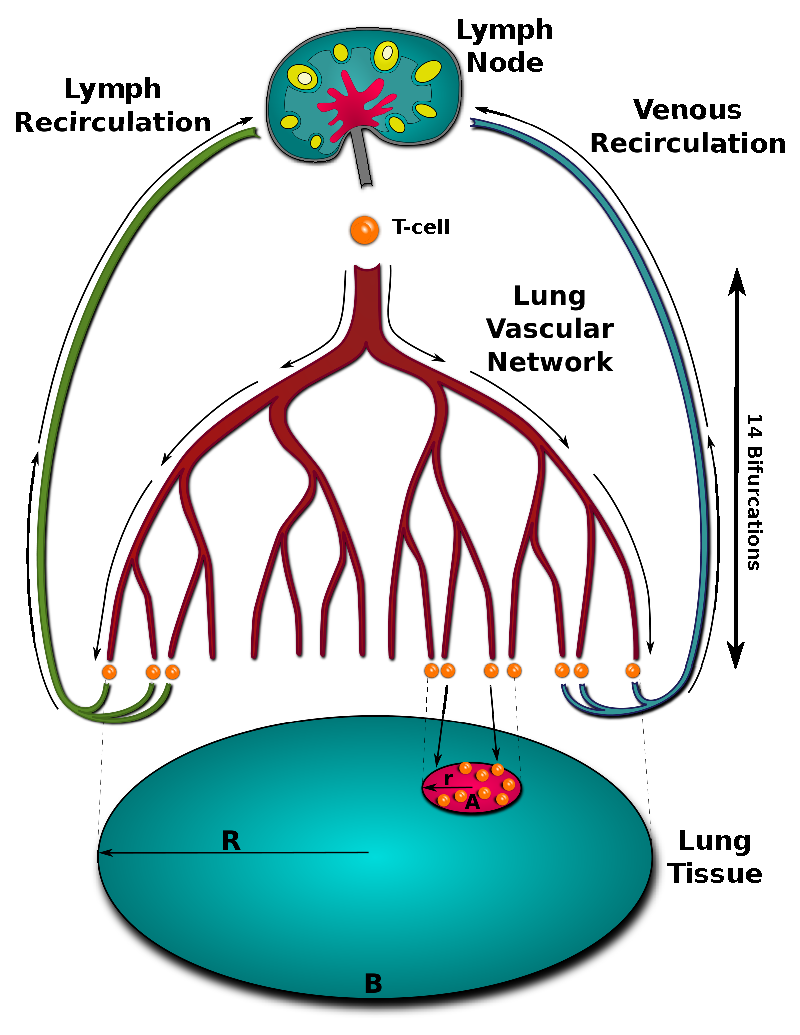
\includegraphics[width=0.5\textwidth]{SystemChart}
\end{center}
\caption{Model of T cell search.  Activated T cells originate in the lymph node and enter the bloodstream after which they randomly navigate through the 14 layers of the branching bronchial network.  Upon reaching a capillary, T cells exit into tissue if cytokine signal is present.  In the absence of signal, the T cell recirculates either through the lymph network or through the pulmonary vein back to the top of the network.}
\label{fig:systemchart}
\end{figure}

\begin{figure}[ht!]
\begin{center}
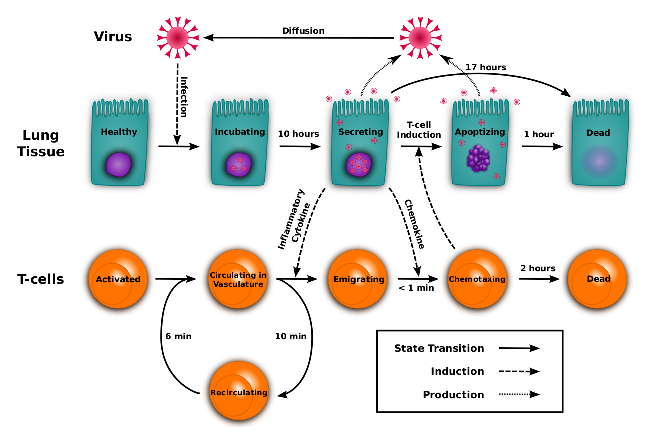
\includegraphics[width=\textwidth]{ModelChart}
\end{center}
\caption{Visual representation of the model.  Healthy epithelial cells infected by virus begin secreting virus after the incubation delay.  Activated T cells traverse the bronchial vascular network and may be recruited by inflammatory cytokine.  Chemotaxing T cells climb the chemokine gradient and induce apoptosis in infected cells.  Solid arrows represent a cell state transition from one behavior to another.  Dashed arrows display the mechanism used to induce a transition.  Dotted arrows indicate the production of new virus.}
\label{fig:modelchart}
\end{figure}


\begin{figure}[ht!]
\begin{center}
 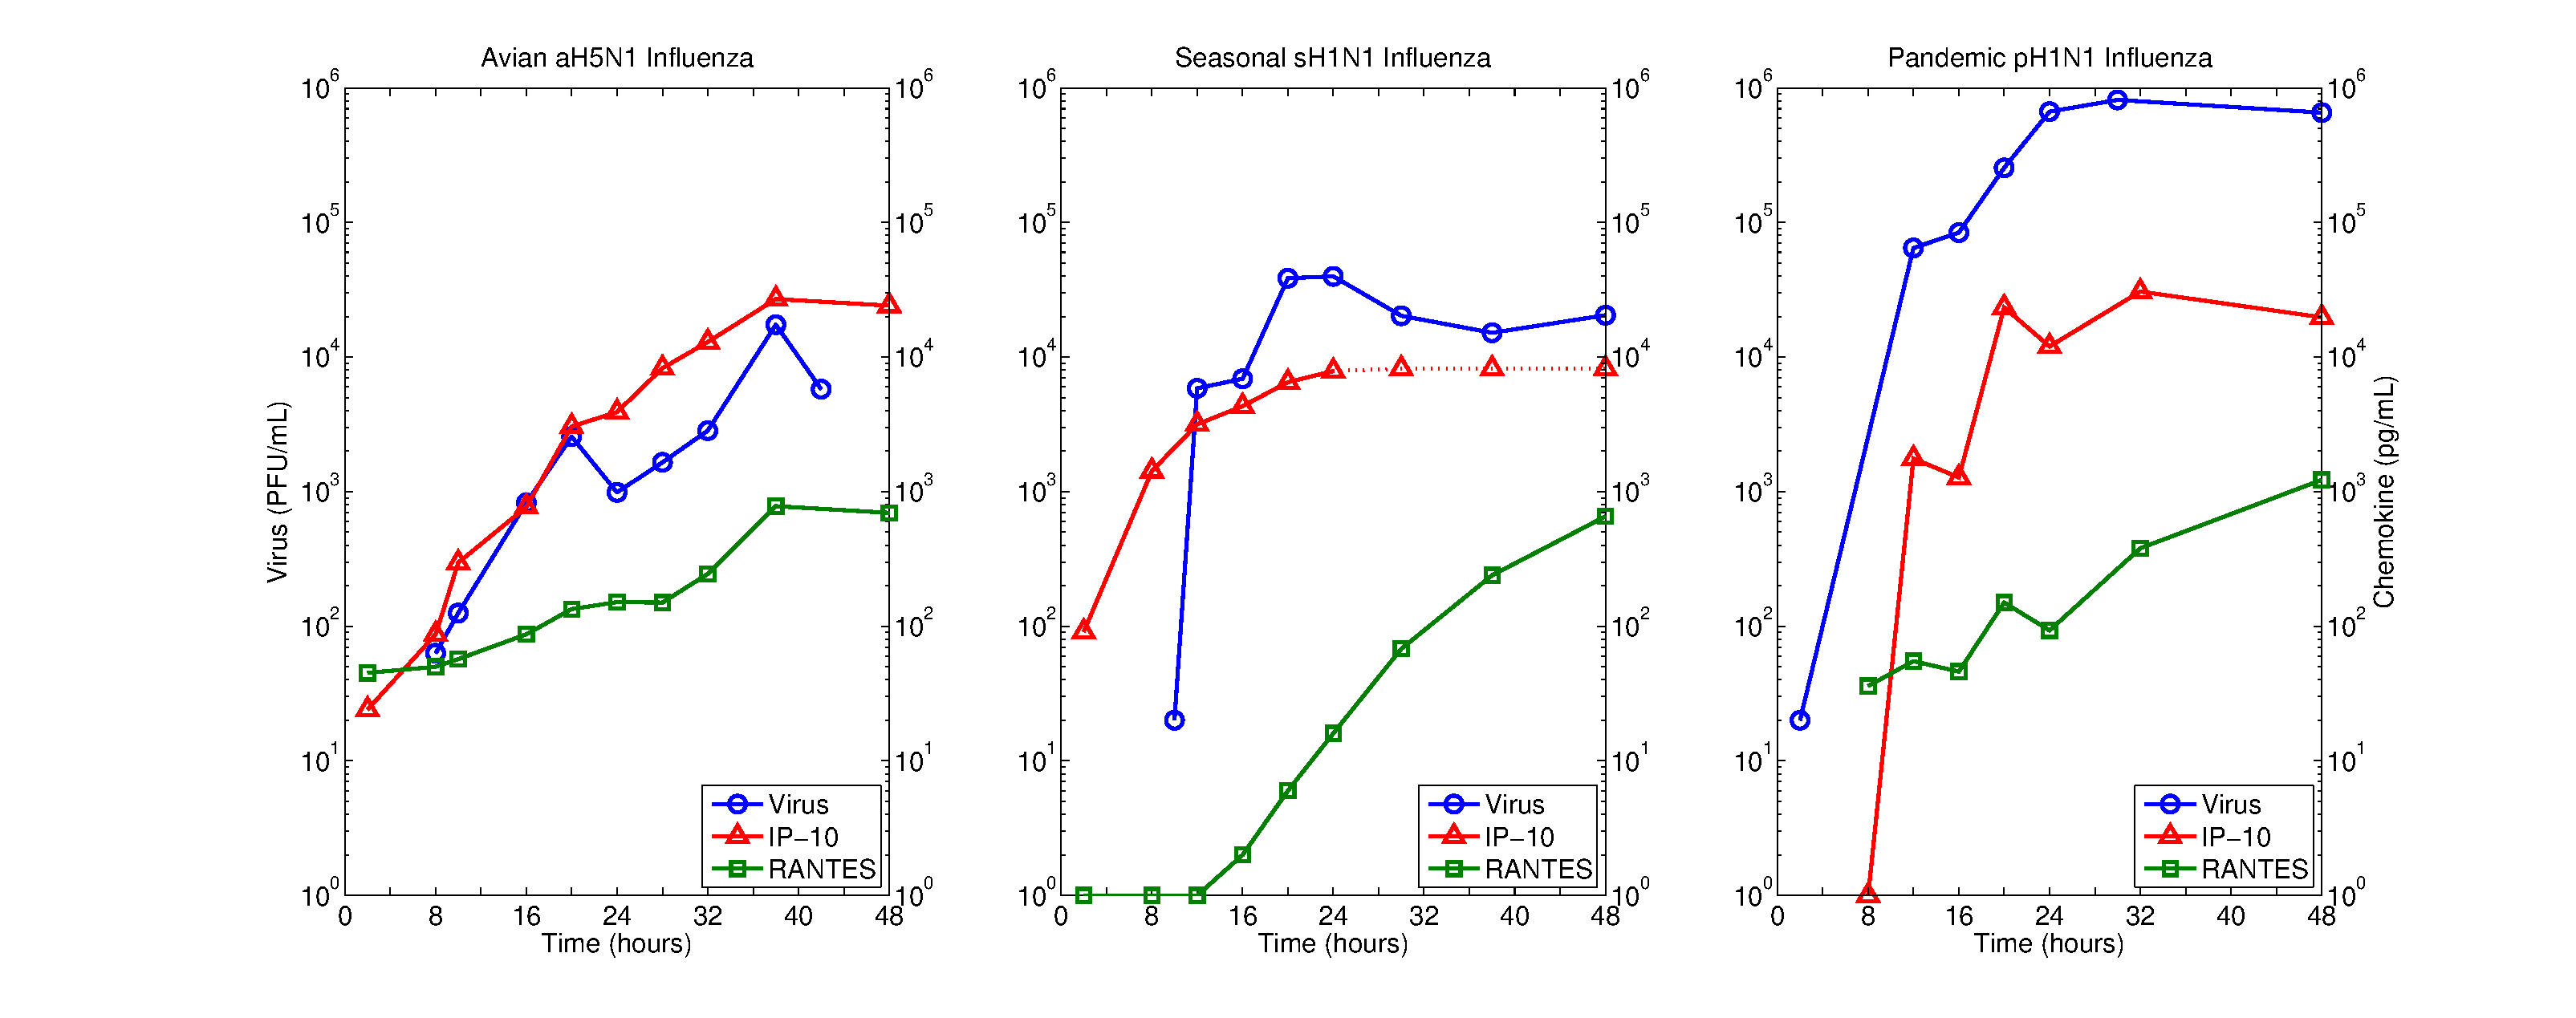
\includegraphics[width=\textwidth]{data}
 \end{center}
\caption{Empirical viral and cytokine titers for three strains of influenza: Avian H5N1, Seasonal sH1N1, and Pandemic pH1N1.  Viral titer (blue circles) is in PFU/mL, and IP-10 (red triangle) and RANTES (green square) are shown in ng/mL.  sH1N1 IP-10 registered three values, not included in model fitting, above the measurement threshold of 8,500 $pg/mL$ (empty red triangles).  Dashed lines show model fits to IP-10 and RANTES data.  Human bronchial epithelial cells were infected at an MOI of 0.01 with one of the three strains of influenza.  Apical fluid for viral secretion and basal media for chemokine secretion was collected at the given time intervals post infection.  Viral culture was performed by a standard plaque assay and chemokine levels were measured using 30 µl aliots for a panel of 17 chemokines and cytokines (not shown).} 
 \label{fig:data}
\end{figure}


\begin{figure}[ht!]
\begin{center}
 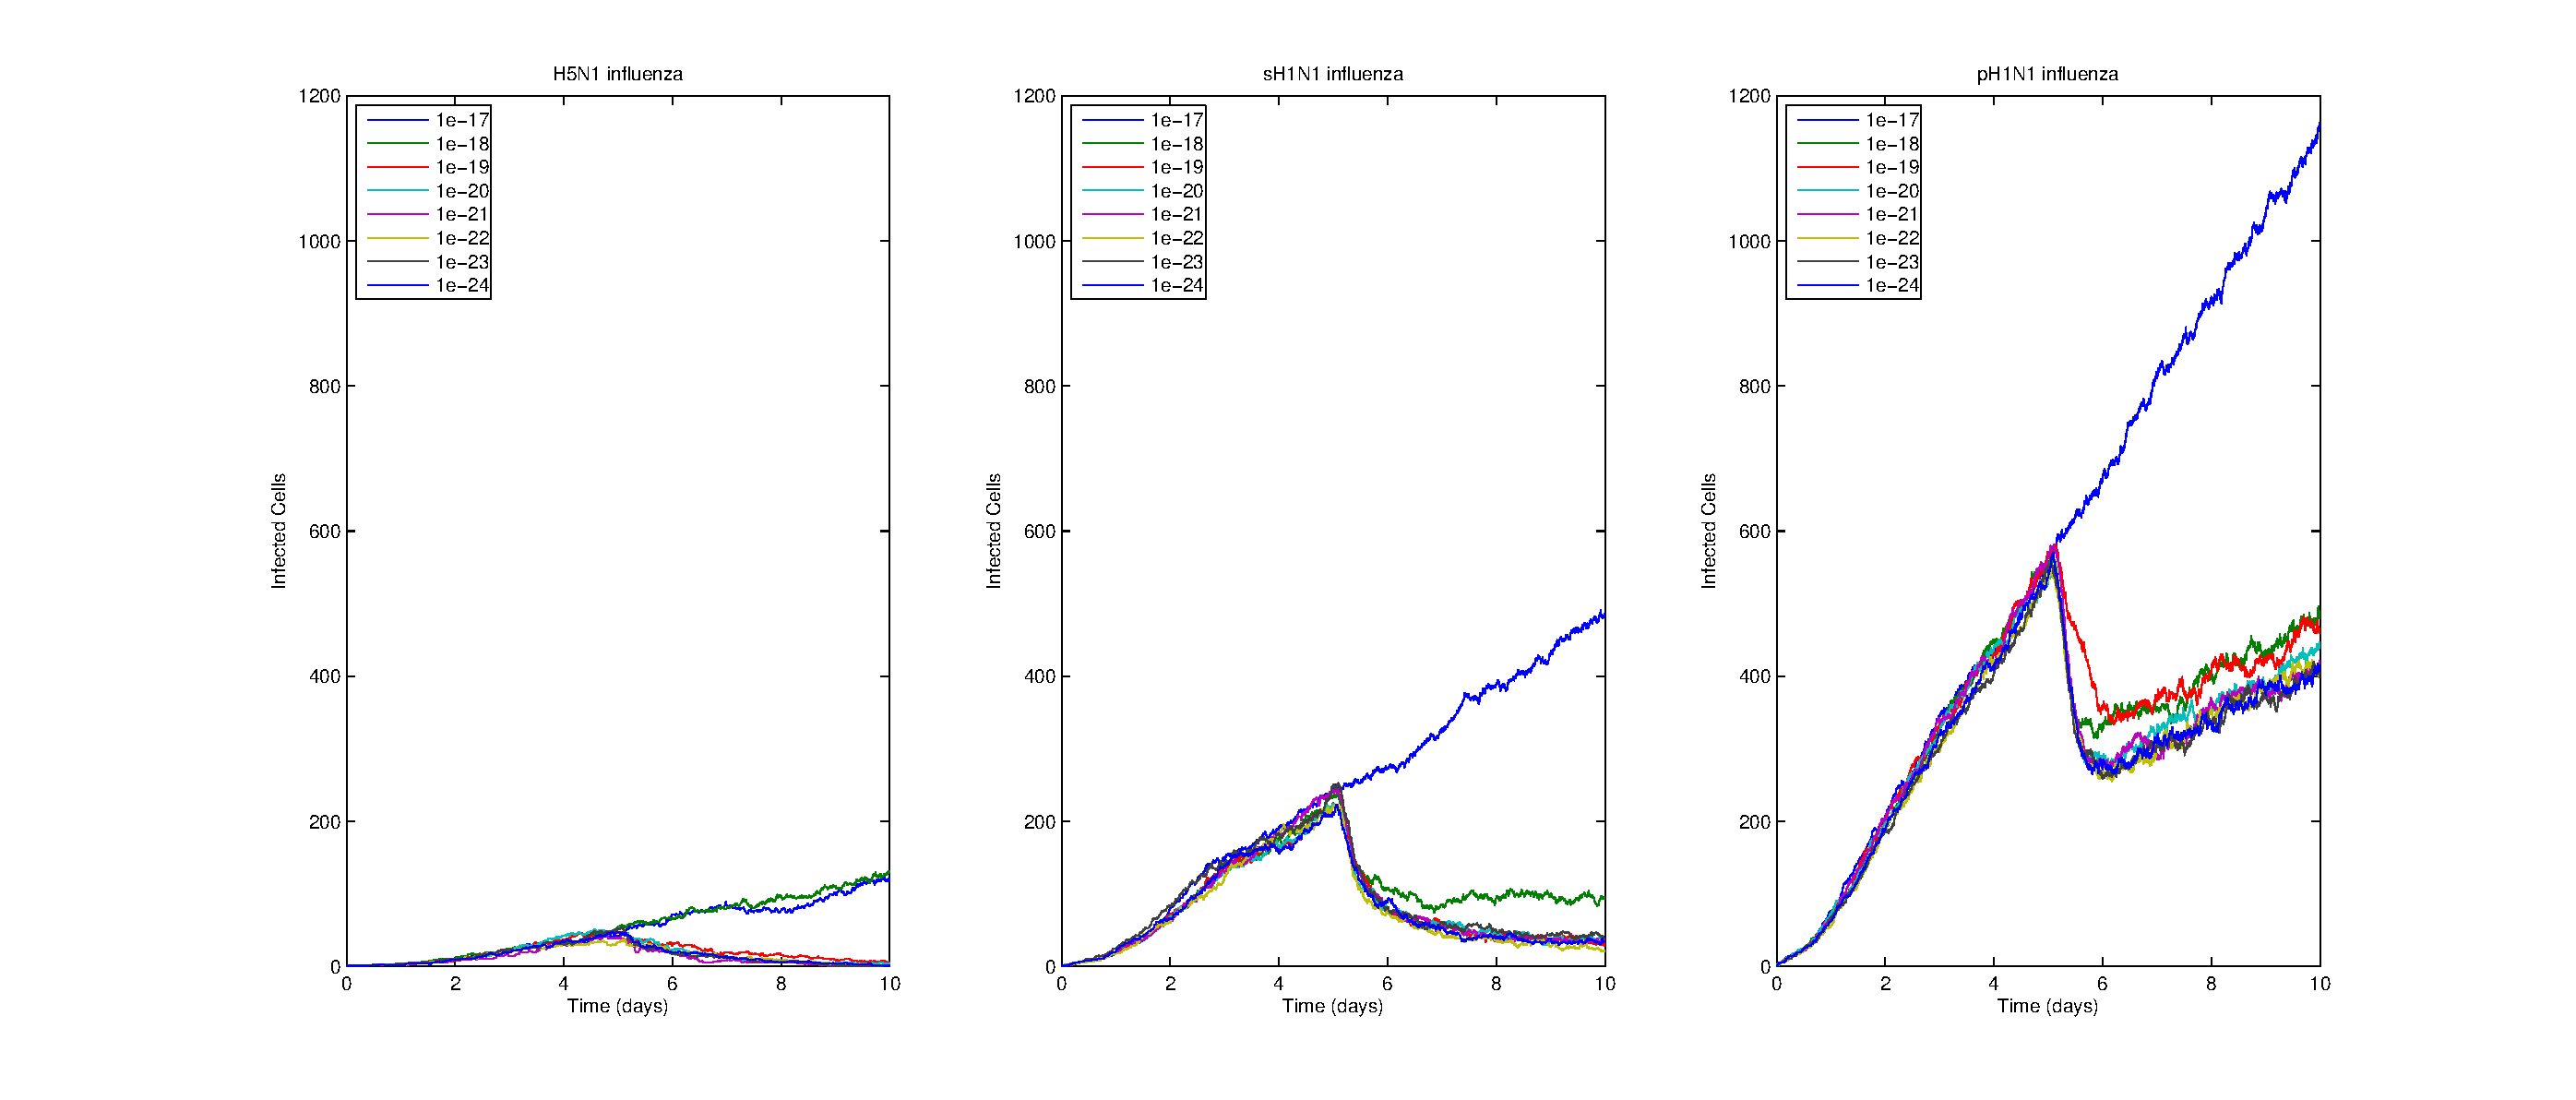
\includegraphics[width=\textwidth]{sensitivity}
 \end{center}
\caption{Varying T cell sensitivity to chemokine: H5N1 model results use RANTES  only, and sH1N1 and pH1N1 use both IP-10 and RANTES. Total number of incubating, secreting and apoptotic cells are plotted for each infection.  The sensitivity value specifies the minimum level of chemokine concentration required for T cells to detect it. } 
 \label{fig:sensitivity}
\end{figure}


\begin{figure}[ht!]
\begin{center}
 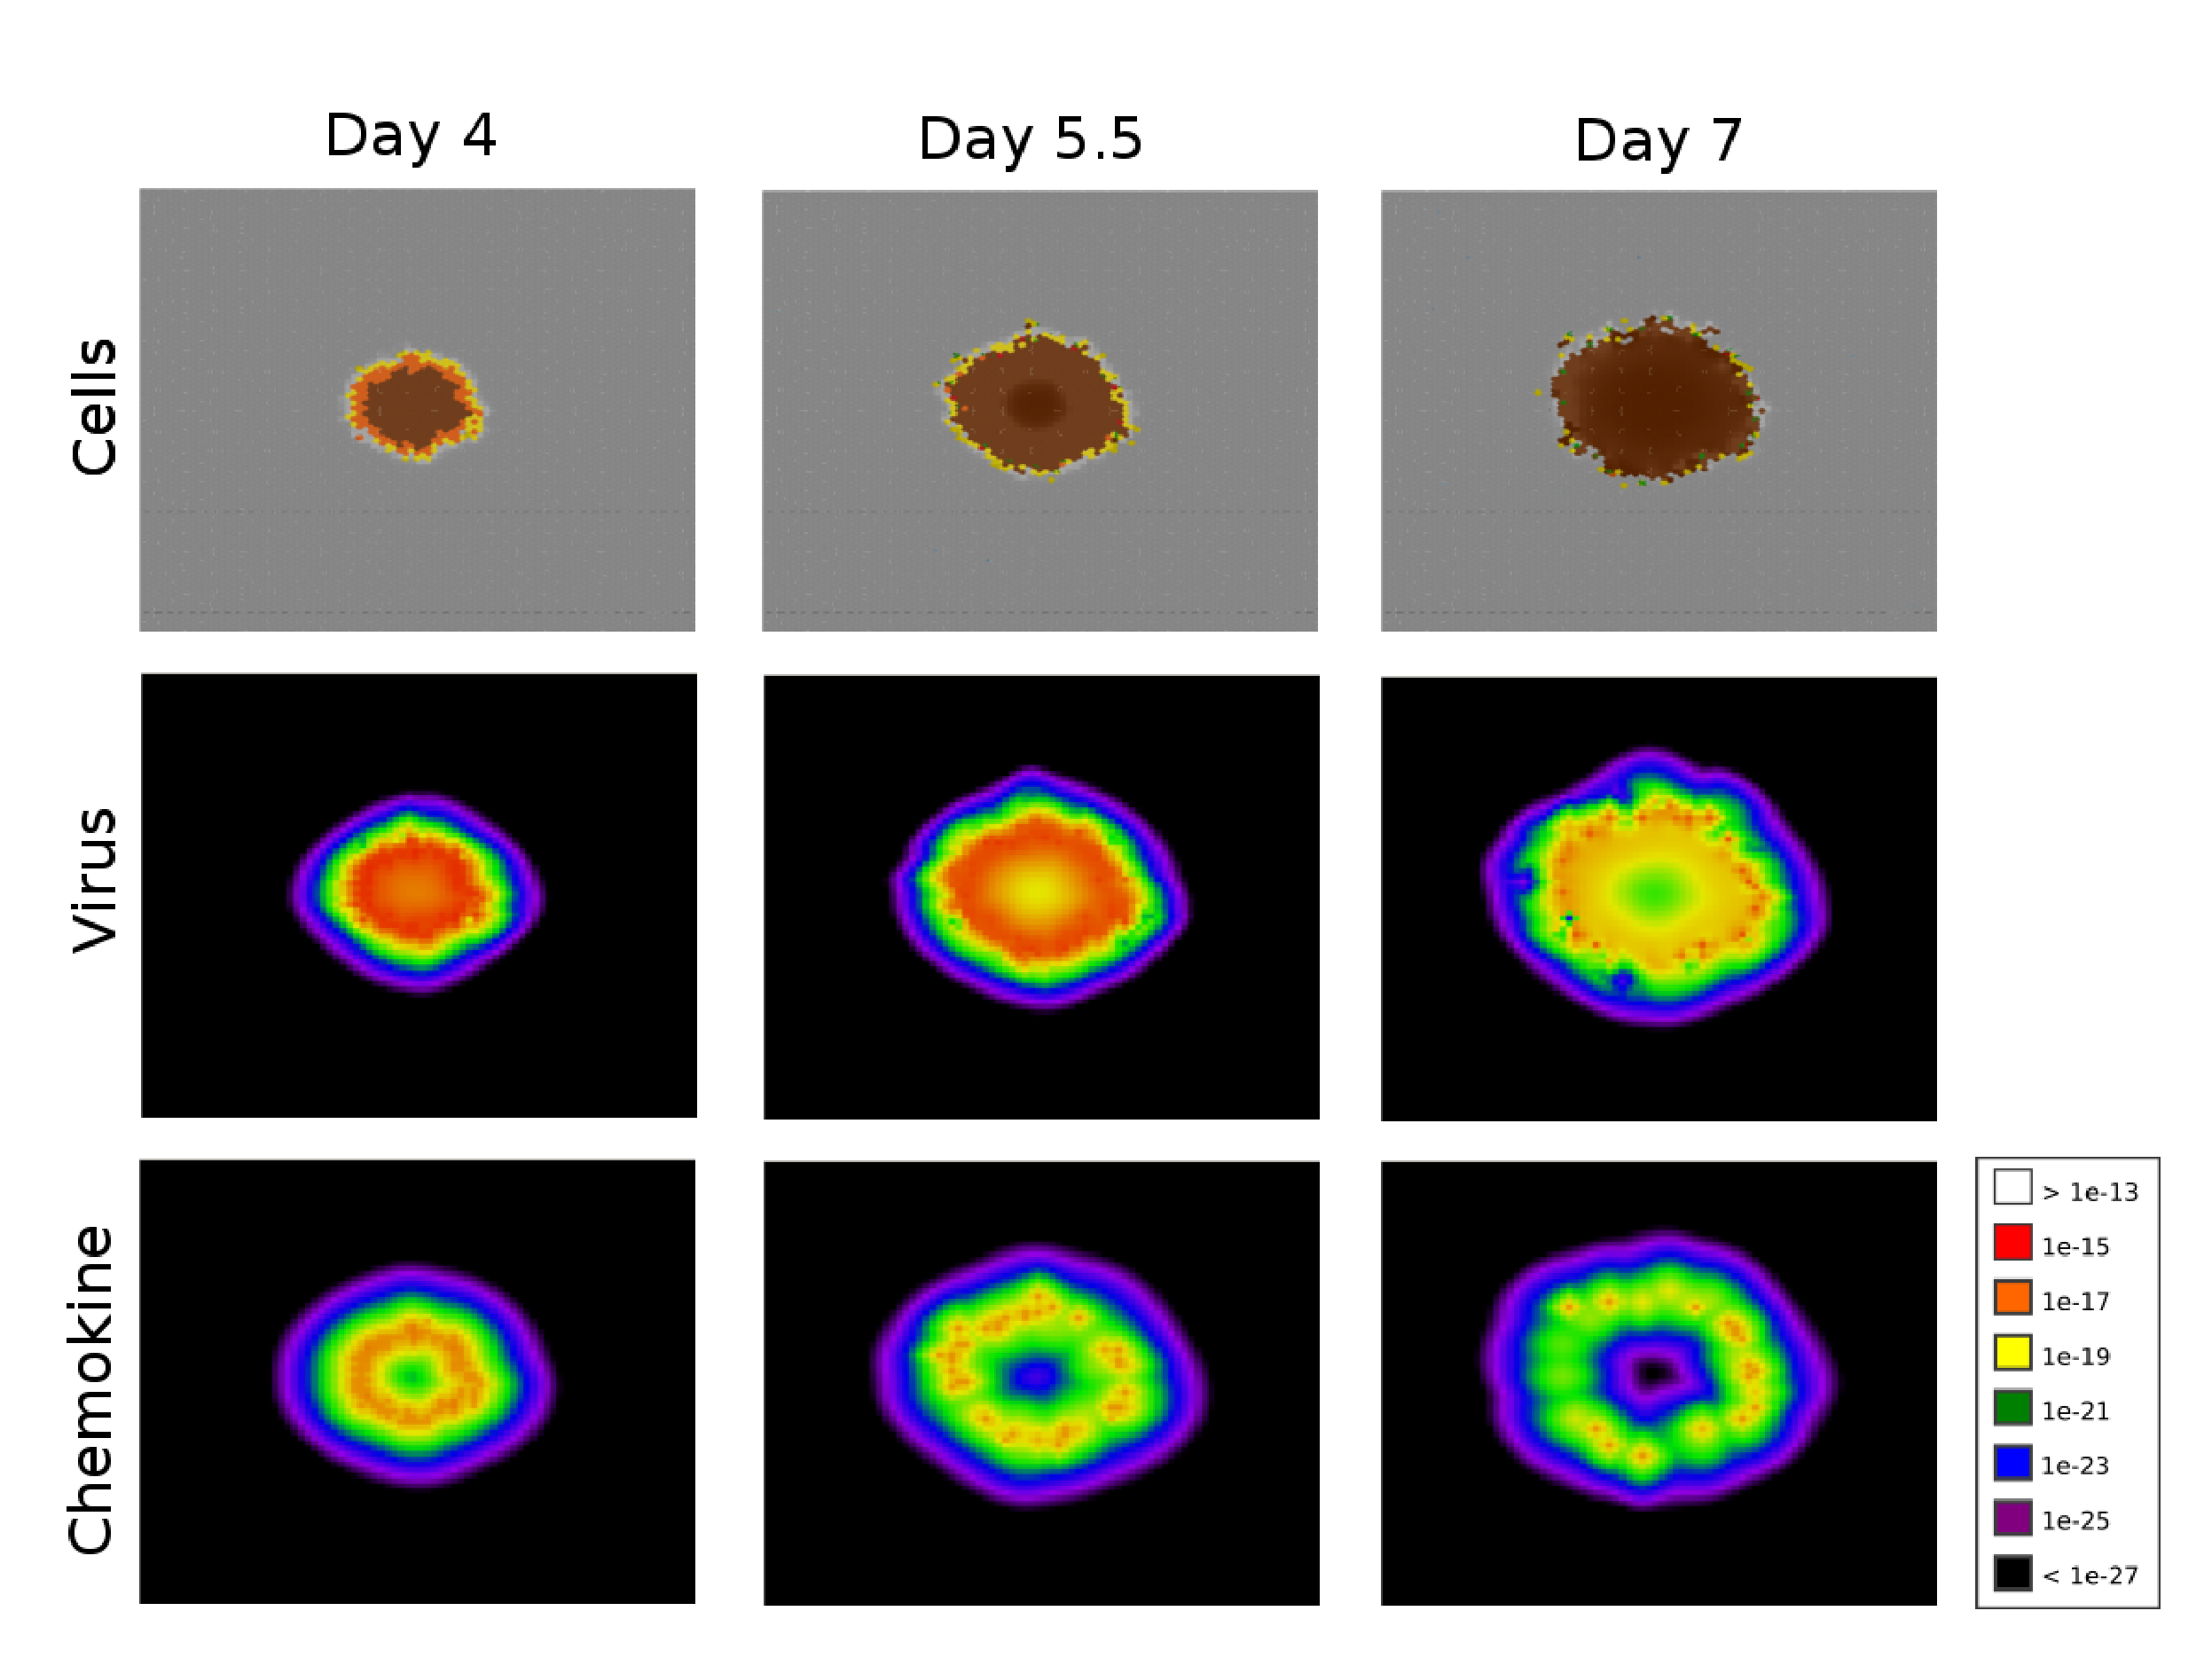
\includegraphics[width=\textwidth]{cycells}
 \end{center}
\caption{Simulated sH1N1 infection. Screenshots from day 4, day 5.5, and day 7.  The top row shows the spreading focus of infection  through the color coding of individual cells:  healthy cells in uninfected tissue (gray),  virus-incubating cells (yellow), virus-secreting cells (orange), apoptotic cells (red), dead cells (brown), and T cells arriving at day 5 (green).  Free virus and chemokine particles are represented by compartmentalized concentrations of mols/mL and ng/mL (see the legend in the bottom right).} 
 \label{fig:cycells}
\end{figure}


\begin{figure}[ht!]
\begin{center}
 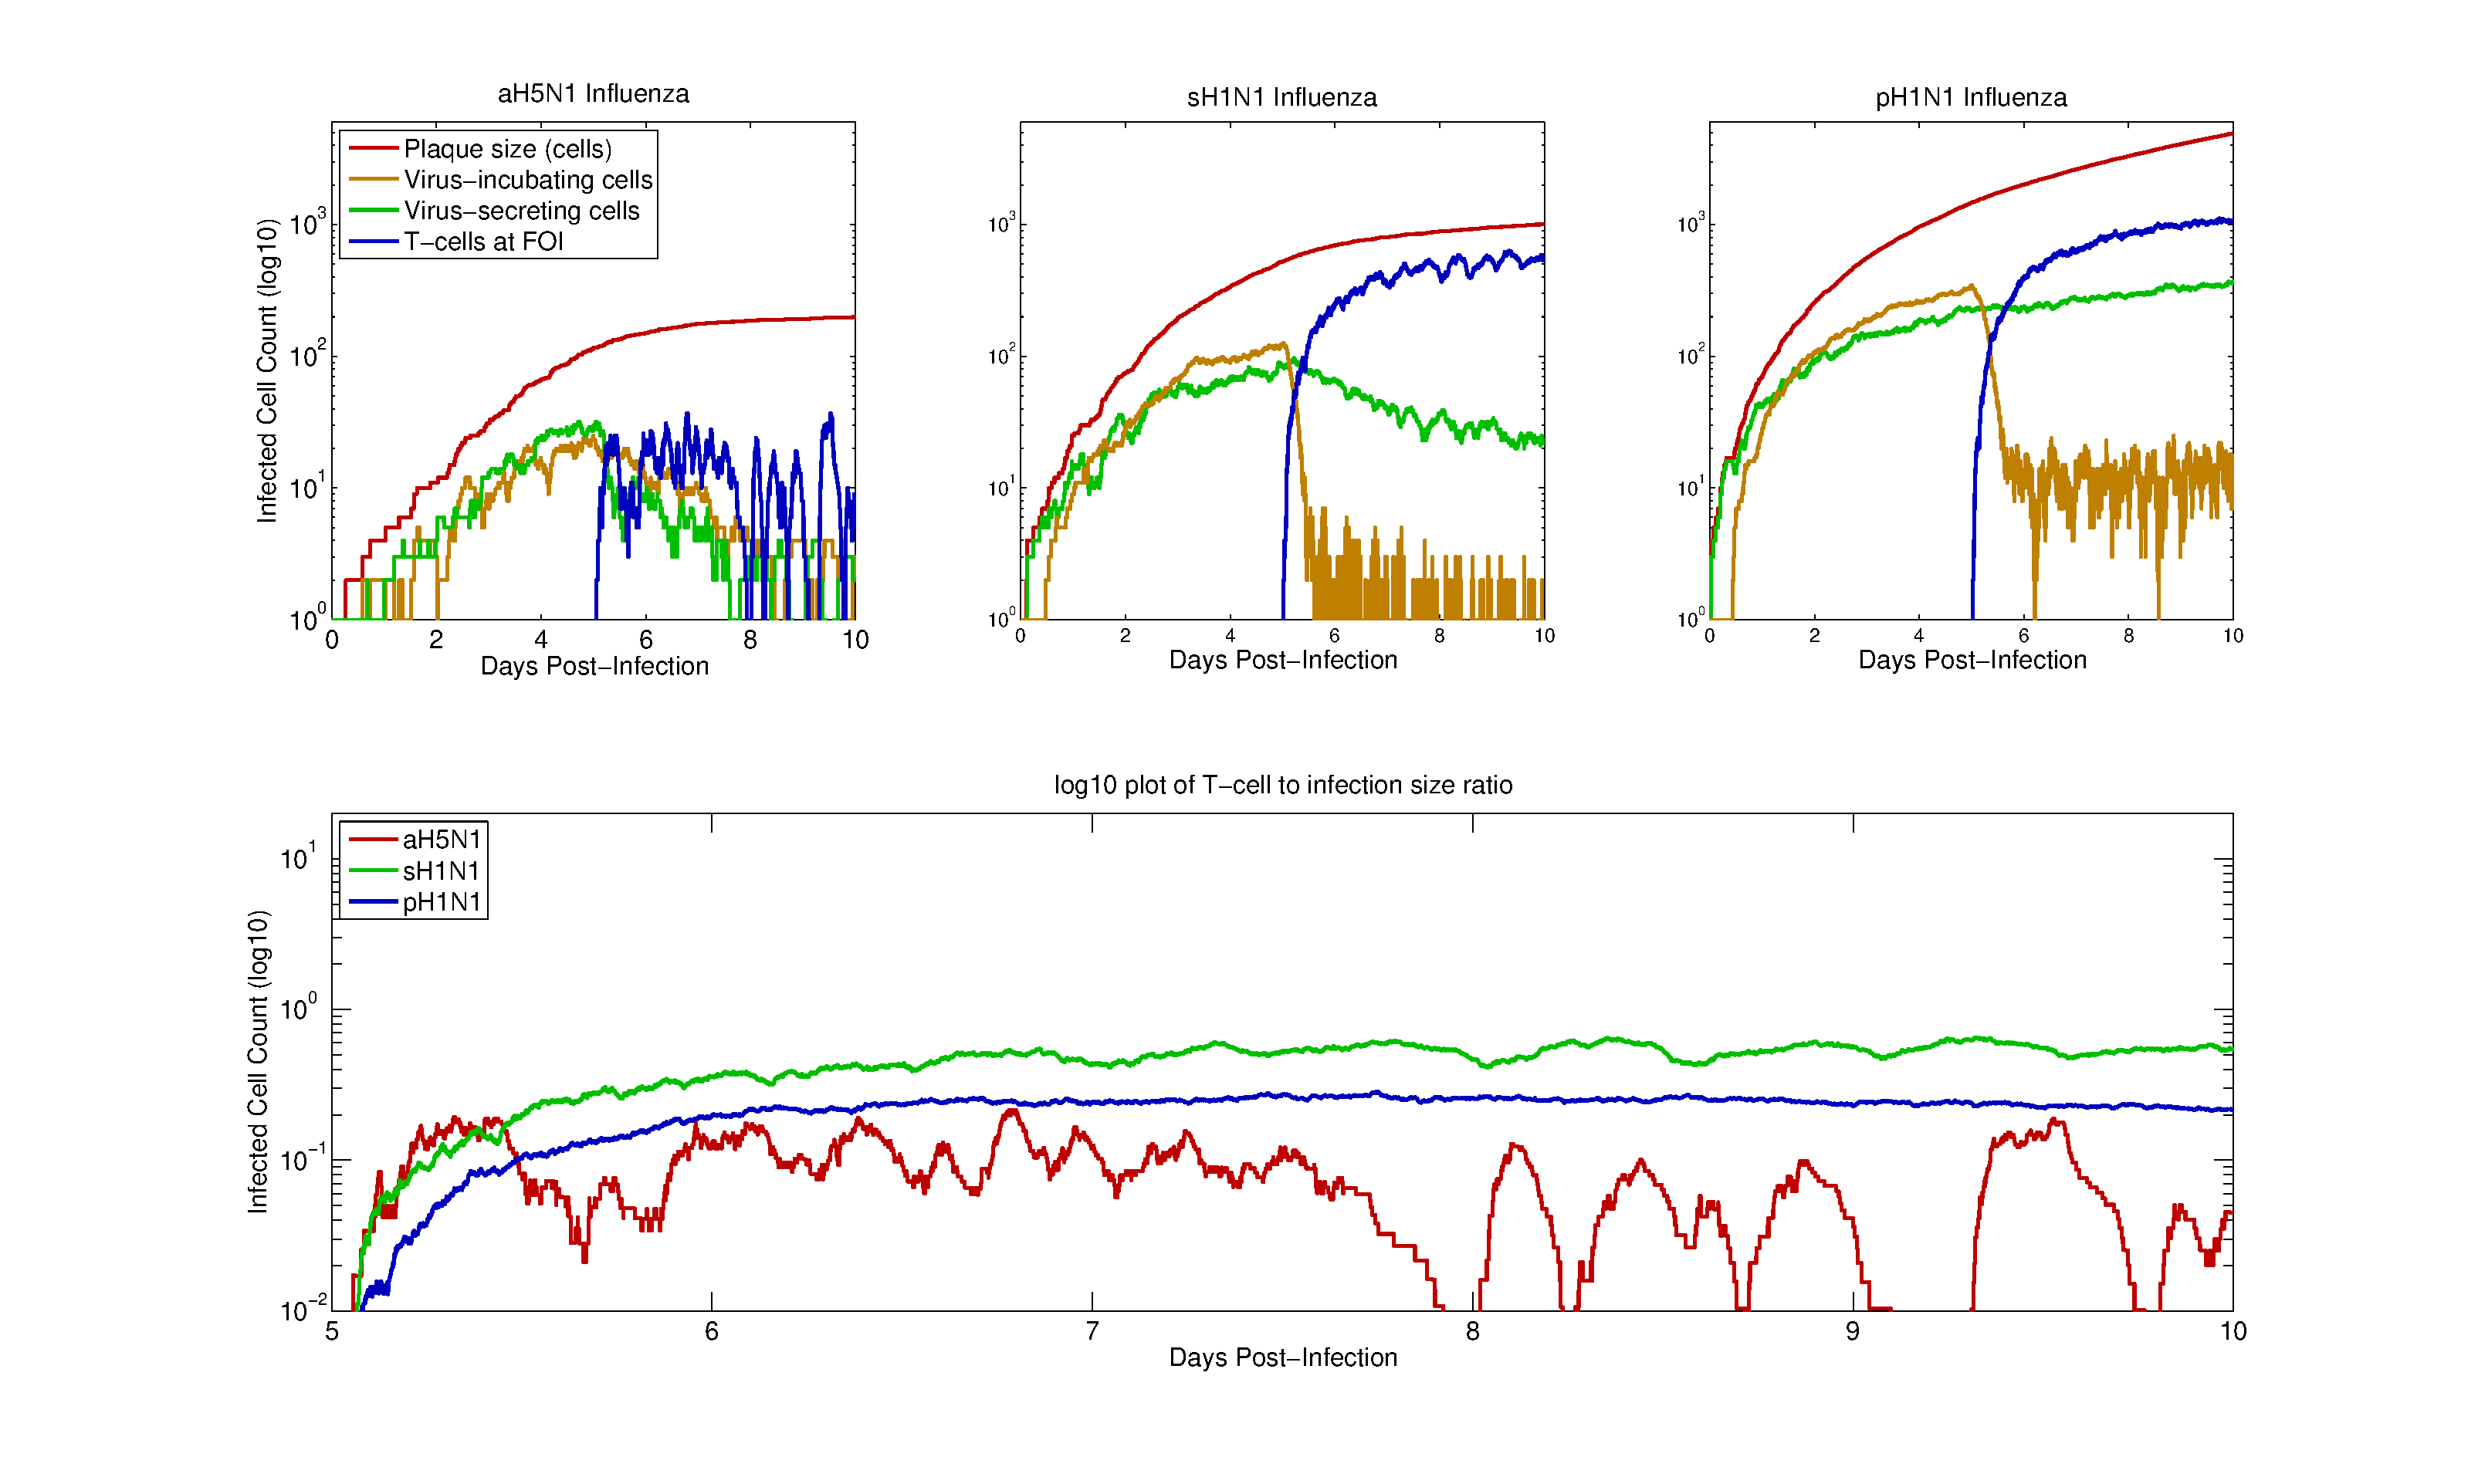
\includegraphics[width=\textwidth]{plaquesize}
 \end{center}
\caption{Comparison of total plaque size (blue), number of virus incubating cells (yellow), number of virus secreting cells (green), and T cells (red) for the simulated infections of aH5N1, sH1N1, and pH1N1.  T cells are able to clear both secreting and incubating cells in aH5N1, are unable to contain incubating cells in sH1N1, and are unable to contain either type of infected cell in pH1N1.  We notice a threshold at day 5: pH1N1 has more expressing cells (green) by a factor of only two to three, yet unlike aH5N1 and sH1N1, the T cell response is unable to clear the expressing population.} 
 \label{fig:plaquesize}
\end{figure}


\section*{Tables}
%\begin{table}[!ht]
%\caption{
%\bf{Table title}}
%\begin{tabular}{|c|c|c|}
%table information
%\end{tabular}
%\begin{flushleft}Table caption
%\end{flushleft}
%\label{tab:label}
% \end{table}


\begin{table}
\begin{center}
\begin{tabular}{ | c | c | c | }
  \hline                        
  Paramter & Value & Source \\
  \hline
  Viral Diffusion in Airway & $.0318 \mu m^2/s$ & \cite{Beauchemin2006} \\
  Viral Decay in Airway &  $1/day$ & \cite{Lee2009} \\
  Chemokine Diffusion Rate & $.318 \mu m^2/s$ & \cite{Beauchemin2006} \\
  Chemokine Decay Rate &  $3.8508\cdot10^{-4}$/s & Selected$^1$\\
  Infection Sensitivity Rate &  $2 hour/virion$ &  Selected$^2$ \\
  Incubation Time &  $10 hours$ & \cite{Mitchell2011} \\
  Expression Time &  $16.7 hours$ & \cite{Mitchell2011}$^3$ \\
  Apoptosis Time & $1 hour$ & \cite{Ganusov2008} \\
  T cell Production Rate & $777/hour$ & \cite{Miao2010} \\ 
  Blood Circulation Time & $6 min$ & \cite{Banerjee2010b} \\
  Search Time In Chemokine-Free Tissue & $10 min$ & \cite{Banerjee2010b} \\
  T Cell Speed (Search) & $30 \mu m/s$ & \cite{Miller2003} \\
  T Cell Speed (Chemotaxis) & $3 \mu m/s$ & \cite{Miller2003} \\
  T Cell Sensitivity to Chemokine & $10 ng/mL$ & \cite{Gao2003} \\
  T Cell Expected Kill Time & $10 min$ & Selected$^4$ \\
  Epithelial Cell Radius & $25 \mu m$ & Selected$^5$ \\
  T Cell Age (at FOI) & $2 hours$ & Selected$^6$ \\
  T Cell Age (in Blood) & $3 days$ & Selected$^6$ \\
  Onset of ATC Lymph Node Exit & $5 days$ & \cite{Banerjee2011} \\
  IgM Strength & Viral decay of $3/day$ & Selected$^7$ \\
  \hline  
\end{tabular}
\caption{Static model parameters.  1) Chosen to correspond to a 30 minute half-life.  2) Epithelial cells are infected at a probabilistic rate such that the expected time for infection in the presence of a single virion is 2 hours.  This scales linearly with the number of virions in the cell's vicinity.  3) Chosen to be a plausible median time (1,000 minutes) between 6 hours and 24 hours.  4) T cells induce apoptosis in nearby virus-secreting epithelial cells at a probabilistic rate such that the expected time to induce apoptosis is 10 minutes.  This rate does not scale with T cell numbers.  5)  The mean surface area of the epithelial cell available for virus contact and entry includes cilia and the radius is estimated to be 25 microns. 6) Parameters chosen after discussions with David Woodland, Trudeau Institute.  7) IgM presence is abstracted by increasing viral decay by a factor of three. }
\label{table:parameters}
\end{center}
\end{table}



\begin{table}
\centering
\begin{tabular}{ | r | c | c | c | }
  \hline                        
  \multicolumn{1}{|c|}{\multirow{2}{*}{Strain}} & IP-10 Production & RANTES Production & Viral Production \\
   & \footnotesize{$(pg/s\cdot cell)$}  & \footnotesize{$(pg/s\cdot cell)$} &  \footnotesize{$(PFU/s\cdot cell)$} \\
  \hline
  \multirow{2}{*}{Avian H5N1} & 2.0e-4 &  1.3e-5 & 5.4e-5 \\
   &  \footnotesize{8.4e-5 --- 4.2e-4} & \footnotesize{7.9e-6 --- 1.9e-5} & \footnotesize{4.4e-5 --- 3.7e-4}\\ 
   \hline
  \multirow{2}{*}{Seasonal H1N1} & 1.8e-4 &  8.9e-7 & 3.8e-4 \\
   & \footnotesize{1.2e-4 --- 3.0e-4} & \footnotesize{4.8e-7 --- 1.6e-6} & \footnotesize{2.8e-4 --- 1.5e-3}\\
   \hline
  \multirow{2}{*}{Pandemic H1N1} & 8.7e-5 &  4.3e-6 & 5.1e-3 \\
   & \footnotesize{1.7e-5 --- 7.1e-4} & \footnotesize{5.0e-7 --- 3.5e-5} & \footnotesize{2.8e-3 --- 5.3e-3} \\
  \hline
\end{tabular}
\caption{Strain-specific model parameters.  Small text values show 95\% confidence intervals resulting from 1,000 bootstrapping runs for each parameter \cite{Wu1986}.  Viral production values are taken from \cite{Mitchell2011}.}
\label{table:strains}
\end{table}


\end{document}

